% ---
\documentclass{article}


% Packages
% ---
\usepackage{amsmath,amssymb,amsthm} 	% Advanced math typesetting
% \usepackage[utf8]{inputenc} 	% Unicode support (Umlauts etc.)
\usepackage[USenglish]{babel} 	% Change hyphenation rules
\usepackage{hyperref} 				% Add a link to your document
\usepackage{graphicx}				% Add pictures to your document
\graphicspath{ {./images/} }	% image directory
\usepackage{listings} 				% Source code formatting and highlighting
\lstset{basicstyle=\ttfamily}		%Typewriter font for code writing
\usepackage{geometry}
\geometry{margin=1in}
\usepackage{enumitem}
\usepackage{float}
%\floatstyle{boxed}
\restylefloat{figure}
\usepackage{mathabx}

\theoremstyle{definition}
\newtheorem{definition}{Def}

\theoremstyle{example}
\newtheorem{example}{Example}

\usepackage{tikz}						% Graph drawing tools
\usetikzlibrary {positioning}

\usepackage{breqn}
\usepackage{multicol} 				% Multiple column functionality
\usepackage{blindtext}


\begin{document}

\author{Jeremi Do Dinh - 61985628}
\title{{\bf CPSC 322}\\ {\it Week II}}
\date{\today}
\maketitle{}


\section*{Lecture IV}


\subsection*{Comparing Searching Algorithms}

\theoremstyle{definition}
\begin{definition}
	A search algorithm is {\bf complete} if, whenever at least one solution exists, the algorithm is {\bf guaranteed to find a solution} within a {\bf finite amount of time}.
\end{definition}
\begin{definition}
	A search algorithm is {\bf optimal} if, when it returns a solution, it is the best solution (i.e. there is no better solution)
\end{definition}

\begin{definition}
	The {\bf time complexity} of a search algorithm is an expression for the {\bf worst-case amount of time} it will take to run
	\begin{itemize}
		\item expressed in terms of the maximum path length $ m $ and the maximum branching factor $ b $.
	\end{itemize}
\end{definition}


\begin{definition}
	The {\bf space complexity} of a search algorithm is an expression for the {\bf worst-case amount of memory} that the algorithm will use (number of paths)
	\begin{itemize}
		\item also expressed in terms of m and b.
	\end{itemize}
\end{definition}

\subsection*{Depth-first Search: DFS}

Depth-first search treats the frontier as a stack. It always selects the path most recently added to the frontier.

\begin{example} 
	\begin{itemize}
		\item The frontier is $ [p_1, p_2, ..., p_r] $
		\item neighbors of last node of $ p_1 $ (its end) are $ \{n_1, ..., n_k\} $
	\end{itemize}
What happens:
\begin{itemize}
	\item $ p_1 $ is selected, and its end is tested for being a goal. If it is not...
	\item New paths are created attaching $ \{n_1, ..., n_k\} $ to $ p_1 $
	\item These “replace” $ p_1 $ at the beginning of the frontier.
	\item Thus, the frontier is now $ [(p_1, n_1), ..., (p_1, n_k), p_2, ..., p_r] $ .
	\item NOTE: $ p_2 $ is only selected when all paths extending $ p_1 $ have been explored.
\end{itemize}
\end{example}
\subsubsection*{Analysis of DFS Summary}
\begin{itemize}
	\item Is DFS complete? {\bf No}
	\begin{itemize}
		\item May not halt on graphs with cycles.
		\item However, DFS is complete for finite acyclic graphs.
	\end{itemize}
\item Is DFS optimal? No
\begin{itemize}
	\item It may stumble on a suboptimal solution first
\end{itemize}
\item What is the time complexity, if the maximum path length is $ m $ and the maximum branching factor is $ b $ ?
\begin{itemize}
	\item Time complexity is $ O(b^m) $: may need to examine every node in the tree.
\end{itemize}
\item What is the space complexity?
\begin{itemize}
	\item Space complexity is $ O(bm) $: the longest possible path is m, and for every node in that path we must maintain a “fringe” of size b.
\end{itemize}
\end{itemize}
\subsubsection*{When it is appropriate?}
\begin{multicols}{2}
	{\bf Appropriate}
	\begin{itemize}
		\item Space is restricted (complex state representation e.g., robotics)
		\item There are many solutions, perhaps with long path lengths, particularly for the case in which all paths lead to a solution
	\end{itemize}
		{\bf Inappropriate}
		\begin{itemize}
			\item Cycles
			\item There are shallow solutions 
			\item If you care about optimality
		\end{itemize}
\end{multicols}

\subsection*{Breadth-first Search: BFS}
Breadth-first search treats the frontier as a queue.

\begin{example}
	\begin{itemize}
		\item the frontier is $ [p_1,p_2, ..., p_r] $
	\item neighbors of the last node of p1 are $ \{n_1,...,n_k\}  $
\end{itemize}
 What happens?
	
	\begin{itemize}
	\item $ p_1 $ is selected, and its end tested for being a path to the goal.
	\item New paths are created attaching $ \{n_1,...,n_k\}  $ to $ p_1 $
	\item These follow $ p_r $ at the end of the frontier.
	\item Thus, the frontier is now [p , ..., p , (p , n ), ..., (p , n )].
	\item $ p_2 $ is selected next.
\end{itemize}
\end{example}

\subsubsection*{Analysis of BFS Summary}
\begin{itemize}
	\item Is BFS complete? {\bf Yes}
	\begin{itemize}
		\item Does not get stuck in cycles
	\end{itemize} 
	\item Is BFS optimal? {\bf Yes}
	\begin{itemize}
		\item guaranteed to find the path that involves the fewest arcs(why?)
	\end{itemize}
	\item What is the time complexity, if the maximum path length is $ m $ and the maximum branching factor is $ b $ ?
	\begin{itemize}
		\item Time complexity is $ O(b^m) $: may need to examine every node in the tree.
	\end{itemize}
	\item What is the space complexity?
	\begin{itemize}
		\item Space complexity is $ O(b^m) $: frontier contains all paths of the relevant length (which is $ \leq $ to the shortest path length to a goal node)
	\end{itemize}
\end{itemize}

\subsubsection*{When it is appropriate?}
\begin{multicols}{2}
	{\bf Appropriate}
	\begin{itemize}
		\item space is not a problem
		\item it's necessary to find the solution with the fewest arcs
		\item although all solutions may not be shallow, at least some are
	\end{itemize}
	{\bf Inappropriate}
	\begin{itemize}
		\item space is limited
		\item all solutions tend to be located deep in the tree
		\item eg. Sudoku solver
		\item the branching factor is very large
	\end{itemize}
\end{multicols}

\subsection*{Iterative Deepening Search}
Essence:
\begin{itemize}
	\item Look with {\bf DFS} for solutions at depth 1, then 2, then 3, etc.
	\item If a solution cannot be found at depth $ D $, look for a solution at depth $ D + 1 $.
	\item You need a depth-bounded depth-first searcher.
	\item Given a bound $ B $ you simply assume that paths of length $ B  $ cannot be expanded....
\end{itemize}
\begin{figure}[H]
	\centering
	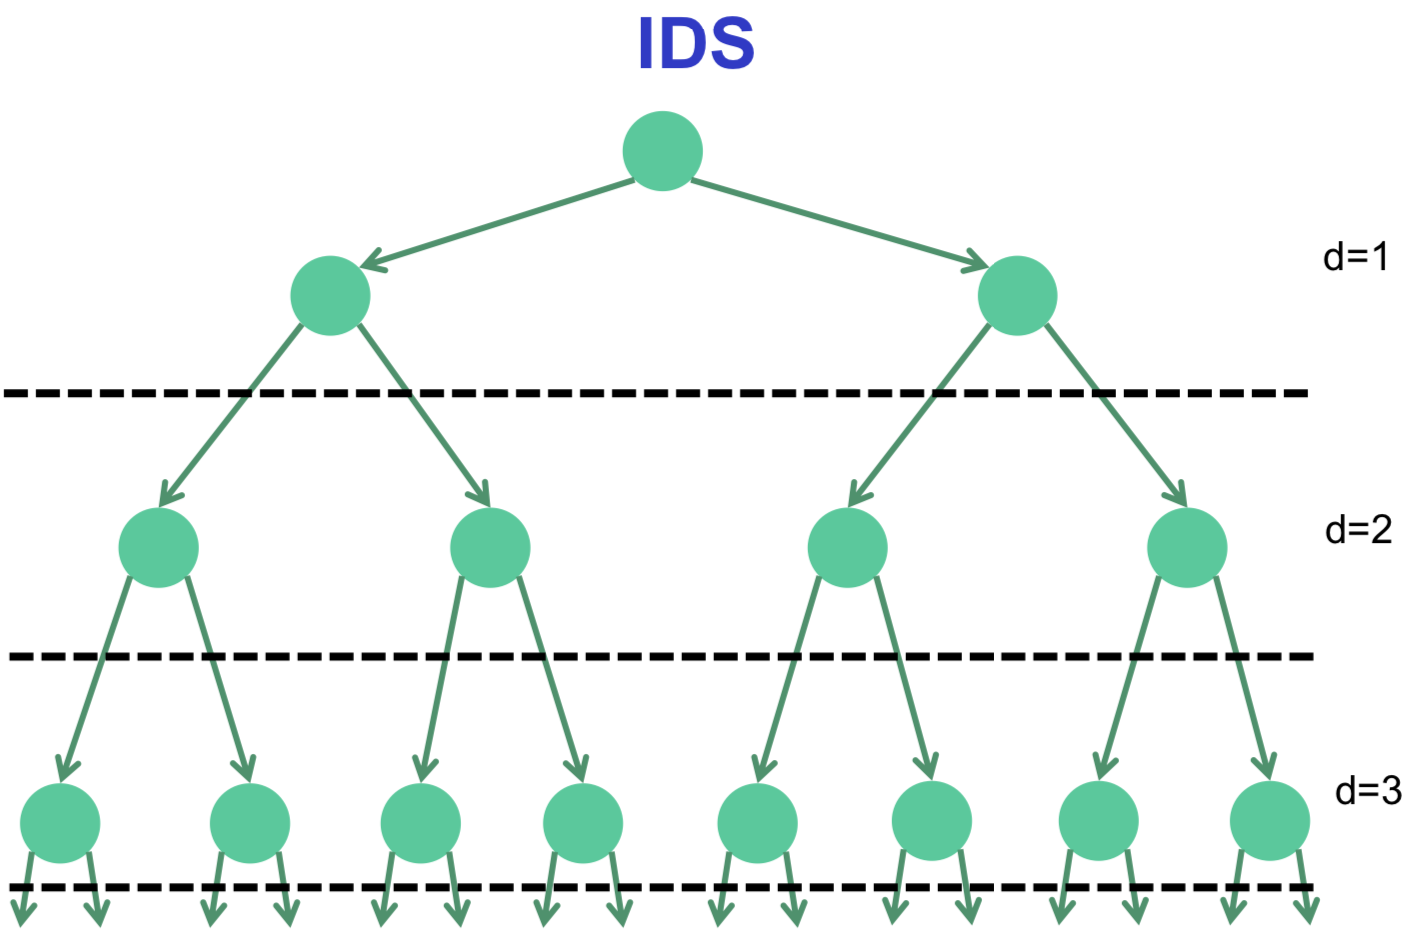
\includegraphics[width = 4in]{pic1}
	\caption{IDS essence}
\end{figure}


\end{document}